\documentclass{article}
\usepackage{xeCJK}
\usepackage{amsmath}
\usepackage{geometry}
\usepackage{graphicx}

\setCJKmainfont{Microsoft YaHei}
\linespread{1.5}
\setlength{\parindent}{0pt}
\geometry{a4paper,scale=0.75}


\begin{document}
\section{第5章}
1.(1)拓广文法如下:
\begin{align*}
    &[1] <S'> \to <S>  \\
    &[2] <S> \to <A> \\
    &[3] <A> \to <B><A> \\
    &[4] <A> \to \epsilon \\
    &[5] <B> \to a<B> \\
    &[6] <B> \to b
\end{align*}
则项目集为: \\
$I_0:$
\begin{align*}
    & <S'> \to .<S>,\quad \# \\
    & <S> \to .<A>,\quad \# \\
    & <A> \to .<B><A>,\quad \# \\
    & <A> \to .,\quad \# \\
    & <B> \to .a<B>,\quad a/b/\# \\
    & <B> \to .b,\quad a/b/\#
\end{align*}
$I_1:$
\begin{align*}
    <S'> \to <S>., \quad \#
\end{align*}
$I_2:$
\begin{align*}
    <S> \to <A>., \quad \#
\end{align*}
$I_3:$
\begin{align*}
    & <A> \to <B>.<A>, \quad \# \\
    & <A> \to .<B><A>, \quad \# \\
    & <A> \to ., \quad \# \\
    & <B> \to .a<B>, \quad a/b/\# \\
    & <B> \to .b, \quad a/b/\#
\end{align*}
$I_4:$
\begin{align*}
    <B> \to b., \quad a/b/\#
\end{align*}
$I_5:$
\begin{align*}
    <B> \to a<B>., \quad a/b/\#
\end{align*}
$I_6:$
\begin{align*}
    & <B> \to a.<B>, \quad a/b/\# \\
    & <B> \to .a<B>, \quad a/b/\# \\
    & <B> \to .b, \quad a/b/\#
\end{align*}
$I_7:$
\begin{align*}
    <A> \to <B><A>., \quad \#
\end{align*}
\\

(2)
根据项目集,构造 $DFA$ 如下:
\begin{figure}[htbp]
    \centering
    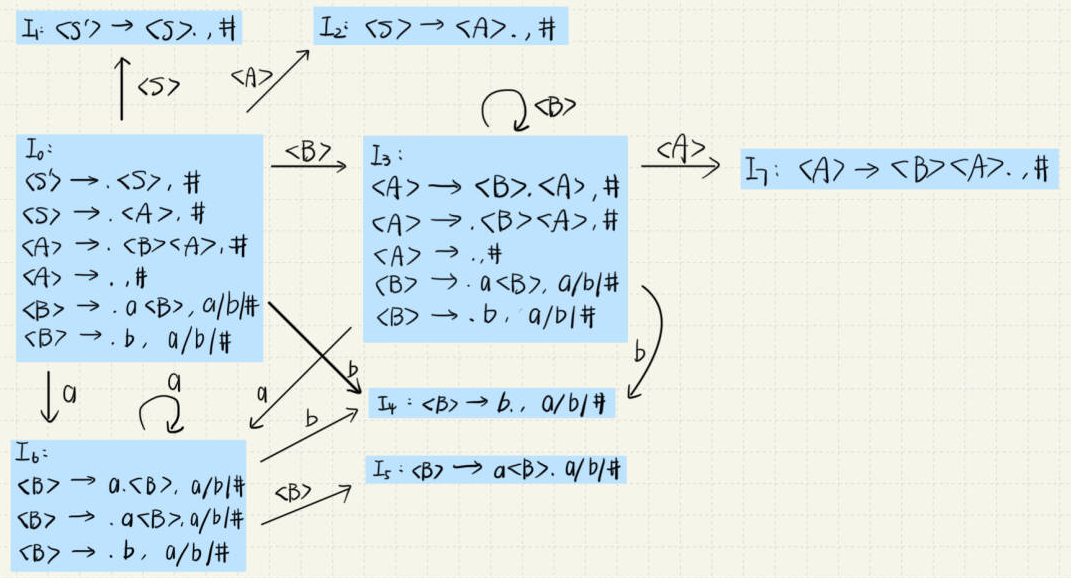
\includegraphics[scale=0.8]{DFA.png}
    \caption{\text{项目集DFA}}
\end{figure}
\newpage
$LR(1)$ 分析表如下:
\begin{table}[h!]
    \begin{center}
        \caption{$LR(1)$ 分析表}
        \setlength{\tabcolsep}{8mm} {
        \begin{tabular}{|l|l|l|l|l|l|l|} 
        \hline
        & \multicolumn{3}{c|}{\textbf{action}} & \multicolumn{3}{c|}{\textbf{goto}} \\
        \hline
        \textbf{state} & \textbf{$a$} & \textbf{$b$} &\textbf{$\#$} & \textbf{$<S>$} & \textbf{$<A>$} & \textbf{$<B>$}\\
        \hline
        0 & s6 & s4 & r4 & 1 & 2 & 3 \\
        \hline
        1 & & & acc & & & \\
        \hline
        2 & & & r2 & & & \\
        \hline
        3 & s6 & s4 & r4 & & 7 & 3 \\
        \hline
        4 & r6 & r6 & r6 & & & \\
        \hline
        5 & r5 & r5 & r5 & & & \\
        \hline
        6 & s6 & s4 & & & & 5\\
        \hline
        7 & & & r3 & & & \\
        \hline
      \end{tabular} 
      }
    \end{center}
\end{table}
\\
(3)分析过程如下:
\newpage
\begin{table}[h!]
    \begin{center}
        \caption{$abab$ 分析过程}
        \setlength{\tabcolsep}{8mm} {
        \begin{tabular}{|l|l|l|l|} 
        \hline
        \textbf{步骤} & \textbf{栈} & \textbf{输入} & \textbf{动作} \\
        \hline
        1 & $0\#$ & $abab\#$ & \text{action}[0,a]=s6 \\
        \hline
        2 & $06\#a$ & $bab\#$ & \text{action}[6,b]=s4 \\
        \hline
        3 & $064\#ab$ & $ab\#$ & \text{action}[4,a]=r6 \\
        \hline
        4 & $06\#a<B>$ & $ab\#$ & \text{goto}[6,<B>]=5 \\  
        \hline
        5 & $065\#a<B>$ & $ab\#$ & \text{action}[5,a]=r5 \\    
        \hline
        6 & $0\#<B>$ & $ab\#$ & \text{goto}[0,<B>]=3 \\
        \hline
        7 & $03\#<B>$ & $ab\#$ & \text{action}[3,a]=s6 \\
        \hline
        8 & $036\#<B>a$ & $b\#$ & \text{action}[6,b]=s4 \\ 
        \hline
        9 & $0364\#<B>ab$ & $\#$ & \text{action}[4,\#]=r6 \\
        \hline
        10 & $036\#<B>a<B>$ & $\#$ & \text{goto}[6,<B>]=5 \\
        \hline
        11 & $0365\#<B>a<B>$ & $\#$ & \text{action}[5,\#]=r5 \\
        \hline
        12 & $03\#<B><B>$ & $\#$ & \text{goto}[3,<B>]=3 \\
        \hline
        13 & $033\#<B><B>$ & $\#$ & \text{action}[3,\#]=r4 \\
        \hline
        14 & $033\#<B><B><A>$ & $\#$ & \text{goto}[3,<A>]=7 \\
        \hline
        15 & $0337\#<B><B><A>$ & $\#$ & \text{action}[7,\#]=r3 \\
        \hline
        16 & $03\#<B><A>$ & $\#$ & \text{goto}[3,<A>]=7 \\
        \hline
        17 & $037\#<B><A>$ & $\#$ & \text{action}[7,\#]=r3 \\
        \hline
        18 & $0\#<A>$ & $\#$ & \text{goto}[0,<A>]=2 \\
        \hline  
        19 & $02\#<A>$ & $\#$ & \text{action}[2,\#]=r2 \\
        \hline
        20 & $0\#<S>$ & $\#$ & \text{goto}[0,<S>]=1 \\
        \hline
        21 & $01\#<S>$ & $\#$ & \text{action}[1,\#]=acc \\
        \hline
        \end{tabular} 
        }
    \end{center}
\end{table}

\newpage

\section{第7章}
1.(1)
\begin{figure}[htbp]
    \centering
    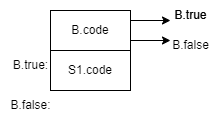
\includegraphics[scale=0.6]{if_then.png}
    \caption{\text{if\_then结构}}
\end{figure}
\\
(2)
\begin{figure}[htbp]
    \centering
    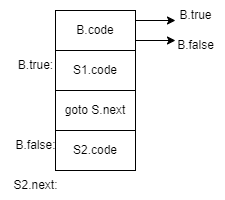
\includegraphics[scale=0.6]{if_then_else.png}
    \caption{\text{if\_then\_else结构}}
\end{figure}
\\
(3)
\begin{figure}[htbp]
    \centering
    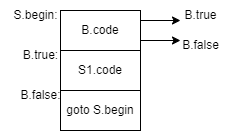
\includegraphics[scale=0.6]{while_do.png}
    \caption{\text{while\_do结构}}
\end{figure}

\newpage
\section{第9章}
1.(1)
\begin{figure}[htbp]
    \centering
    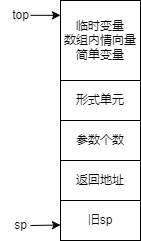
\includegraphics[scale=0.8]{C.png}
    \caption{\text{非嵌套语言活动记录}}
\end{figure}
\\
(2)
\begin{figure}[htbp]
    \centering
    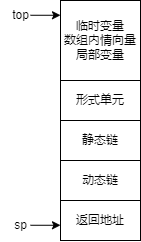
\includegraphics[scale=0.8]{Pascal.png}
    \caption{\text{嵌套语言活动记录}}
\end{figure}


\section{第11章}
1.(1) $2 + 2 + 1 + 2 = 7$ \\
(2) $2 + 2 + 2 + 2 = 8$ \\
(3) $2 + 2 + 2 = 6$ \\
(4) $2 + 2 + 1 + 1 = 6$
\end{document}